\documentclass{ximera}

\author{Bart Snapp}

\title{Plane and sphere}

\begin{document}
\begin{abstract}
  One group member will plot a plane intersecting a sphere.
\end{abstract}
\maketitle

One group member will produce a plot like this one:
\begin{image}
  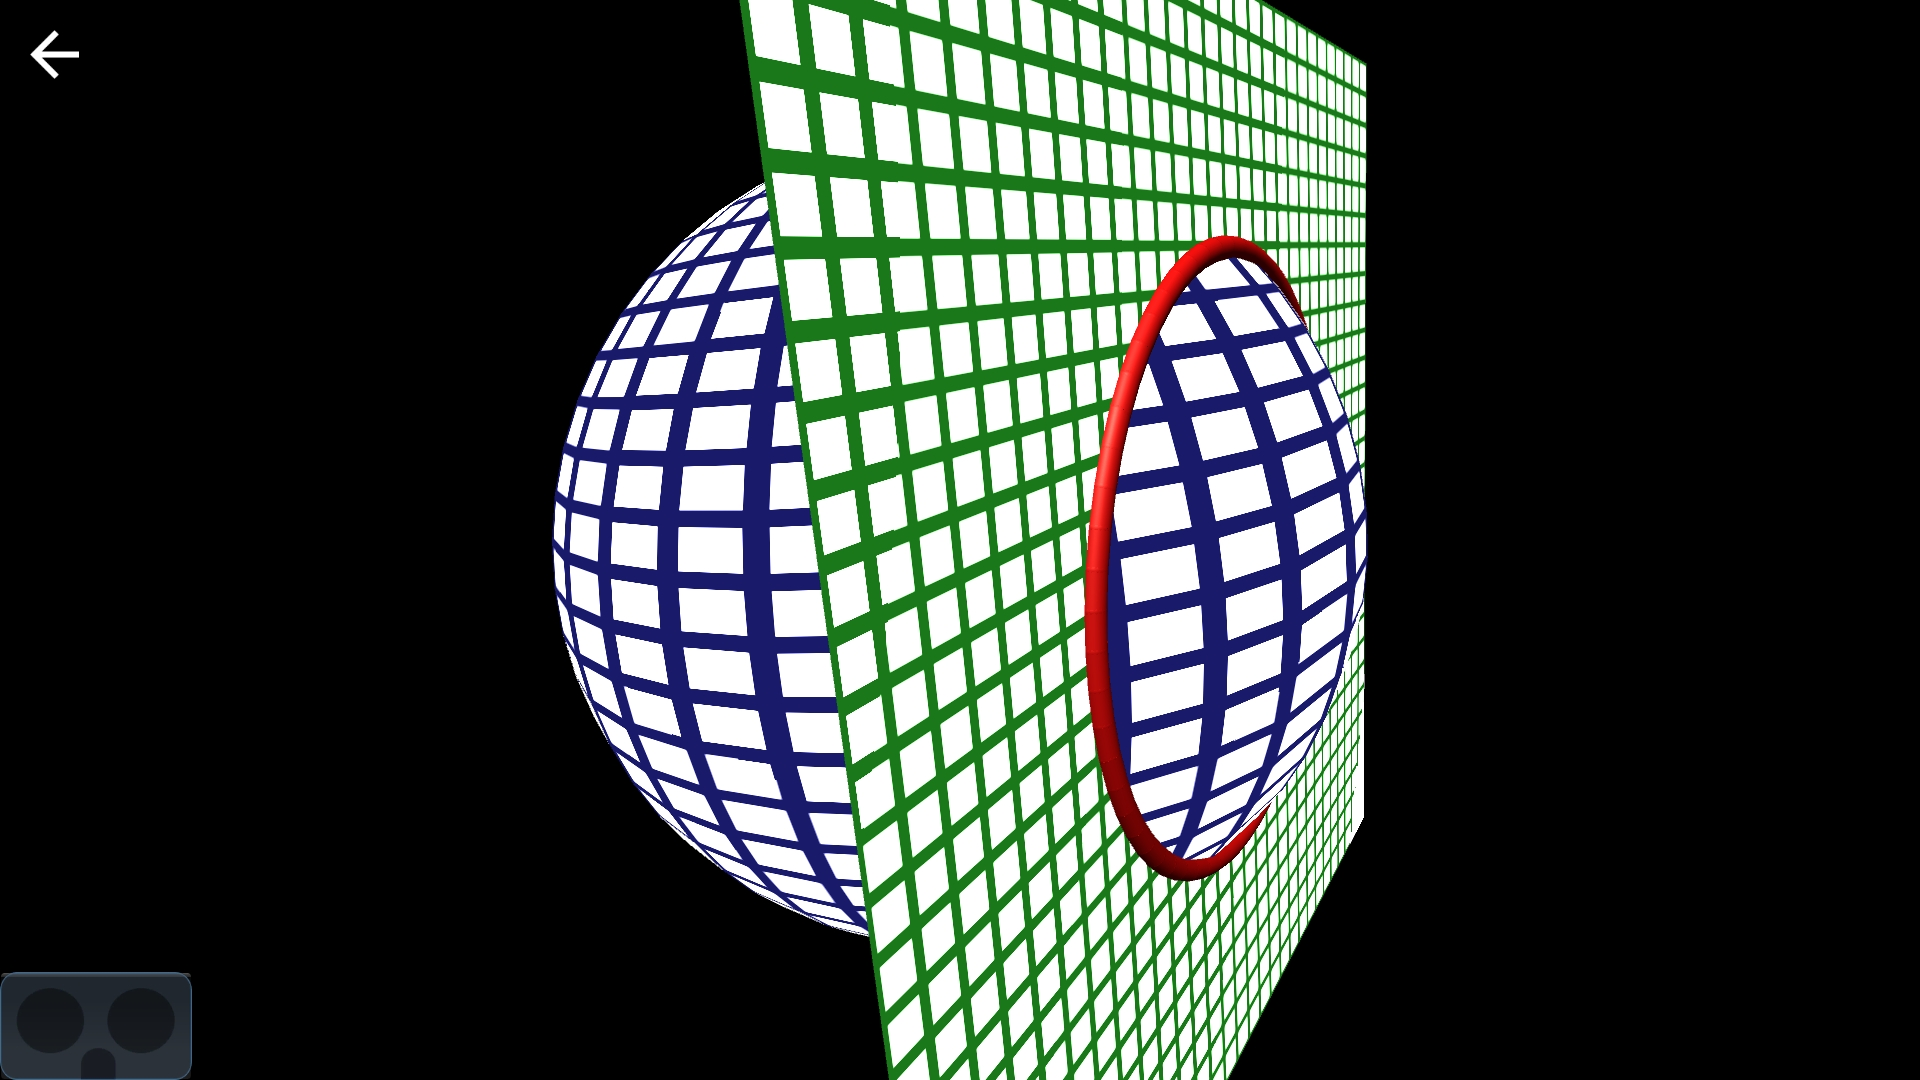
\includegraphics{planeAndSphere.png}
\end{image}

This is the intersection of a sphere of radius $4$ centered at the origin with the plane $x=3$.

You need to reproduce this plot along with a circle at the
intersection.
As a gesture of friendship, I will tell you that the parametric
formula for a sphere of radius $R$ is:
\begin{align*}
  x(s,t) &= R\cdot \cos(t)\sin(s)\\
  y(s,t) &= R\cdot \sin(t)\sin(s)\\
  z(s,t) &= R\cdot \cos(s),
\end{align*}
where $0\le t< 2\pi$ and $0\le s \le \pi$.

You may make the circle indicating the intersection of any color you
wish.
\end{document}
